\documentclass[12pt,onecolumn]{article}
\usepackage[utf8]{inputenc} % UTF8 input encoding
\usepackage[T2A]{fontenc}   % T2A font encoding for Cyrillic script
\usepackage[russian]{babel} % Russian language support
\usepackage{listings}
\usepackage{float}
\usepackage{mathtools}
\usepackage{longtable}
\usepackage{multicol}
\usepackage{lipsum}
\everymath{\displaystyle}
\usepackage{listings} 
\usepackage[usenames]{color}
\usepackage{geometry}
\usepackage{verbatim}

\geometry{
  a4paper,
  top=25mm, 
  right=15mm, 
  bottom=25mm, 
  left=15mm
}

\definecolor{deepgreen}{RGB}{0,100,0}
\lstdefinestyle{sql}{language=SQL, 
  basicstyle=\small\ttfamily,
  commentstyle=\color{deepgreen},
  stringstyle=\color{magenta}\ttfamily,
  keywordstyle=\color{blue},
  numbers=left,
  numberstyle=\scriptsize,
  numbersep=5pt,
  frame=single,
  breaklines=true,
  breakatwhitespace=true,
  showstringspaces=false,
  tabsize=4,
  inputencoding=utf8,
  extendedchars=true,
  literate={а}{{\selectfont\char224}}1
          {б}{{\selectfont\char225}}1
          {в}{{\selectfont\char226}}1
          {г}{{\selectfont\char227}}1
          {д}{{\selectfont\char228}}1
          {е}{{\selectfont\char229}}1
          {ё}{{\"e}}1
          {ж}{{\selectfont\char230}}1
          {з}{{\selectfont\char231}}1
          {и}{{\selectfont\char232}}1
          {й}{{\selectfont\char233}}1
          {к}{{\selectfont\char234}}1
          {л}{{\selectfont\char235}}1
          {м}{{\selectfont\char236}}1
          {н}{{\selectfont\char237}}1
          {о}{{\selectfont\char238}}1
          {п}{{\selectfont\char239}}1
          {р}{{\selectfont\char240}}1
          {с}{{\selectfont\char241}}1
          {т}{{\selectfont\char242}}1
          {у}{{\selectfont\char243}}1
          {ф}{{\selectfont\char244}}1
          {х}{{\selectfont\char245}}1
          {ц}{{\selectfont\char246}}1
          {ч}{{\selectfont\char247}}1
          {ш}{{\selectfont\char248}}1
          {щ}{{\selectfont\char249}}1
          {ъ}{{\selectfont\char250}}1
          {ы}{{\selectfont\char251}}1
          {ь}{{\selectfont\char252}}1
          {э}{{\selectfont\char253}}1
          {ю}{{\selectfont\char254}}1
          {я}{{\selectfont\char255}}1
          {А}{{\selectfont\char192}}1
          {Б}{{\selectfont\char193}}1
          {В}{{\selectfont\char194}}1
          {Г}{{\selectfont\char195}}1
          {Д}{{\selectfont\char196}}1
          {Е}{{\selectfont\char197}}1
          {Ё}{{\"E}}1
          {Ж}{{\selectfont\char198}}1
          {З}{{\selectfont\char199}}1
          {И}{{\selectfont\char200}}1
          {Й}{{\selectfont\char201}}1
          {К}{{\selectfont\char202}}1
          {Л}{{\selectfont\char203}}1
          {М}{{\selectfont\char204}}1
          {Н}{{\selectfont\char205}}1
          {О}{{\selectfont\char206}}1
          {П}{{\selectfont\char207}}1
          {Р}{{\selectfont\char208}}1
          {С}{{\selectfont\char209}}1
          {Т}{{\selectfont\char210}}1
          {У}{{\selectfont\char211}}1
          {Ф}{{\selectfont\char212}}1
          {Х}{{\selectfont\char213}}1
          {Ц}{{\selectfont\char214}}1
          {Ч}{{\selectfont\char215}}1
          {Ш}{{\selectfont\char216}}1
          {Щ}{{\selectfont\char217}}1
          {Ъ}{{\selectfont\char218}}1
          {Ы}{{\selectfont\char219}}1
          {Ь}{{\selectfont\char220}}1
          {Э}{{\selectfont\char221}}1
          {Ю}{{\selectfont\char222}}1
          {Я}{{\selectfont\char223}}1
}
\lstset{style=sql}



\begin{document}
\setcounter{tocdepth}{4}
\begin{center}
    Федеральное государственное автономное образовательное учреждение высшего образования "Национальный Исследовательский Университет ИТМО"\\ 
    Мегафакультет Компьютерных Технологий и Управления\\
    Факультет Программной Инженерии и Компьютерной Техники \\
    
\includegraphics[scale=0.3]{image/itmo.jpg} % нужно закинуть картинку логтипа в папку с отчетом
\end{center}
\vspace{1cm}


\begin{center}
    \textbf{Лабораторная работа №3}\\
    по дисциплине\\
    \textbf{'Информационные системы и базы данных'}\\
    \textbf{Вариант 564738291}
\end{center}

\vspace{2cm}

\begin{flushright}
  Выполнил Студент  группы P33102\\
  \textbf{Лапин Алексей Александрович}\\
  Преподаватель: \\
  \textbf{Сагайдак Алина Алексеевна}\\
\end{flushright}

\vspace{6cm}
\begin{center}
    г. Санкт-Петербург\\
    2023г.
\end{center}

\newpage
\tableofcontents
\newpage

\section{Текст задания.}
Составить запросы на языке SQL (пункты 1-2).\\
Для каждого запроса предложить индексы, добавление которых уменьшит время выполнения запроса (указать таблицы/атрибуты, для которых нужно добавить индексы, написать тип индекса; объяснить, почему добавление индекса будет полезным для данного запроса).\\
Для запросов 1-2 необходимо составить возможные планы выполнения запросов. Планы составляются на основании предположения, что в таблицах отсутствуют индексы. Из составленных планов необходимо выбрать оптимальный и объяснить свой выбор.
Изменятся ли планы при добавлении индекса и как?\\
Для запросов 1-2 необходимо добавить в отчет вывод команды EXPLAIN ANALYZE [запрос]\\
Подробные ответы на все вышеперечисленные вопросы должны присутствовать в отчете (планы выполнения запросов должны быть нарисованы, ответы на вопросы - представлены в текстовом виде).\\
\begin{verbatim}
1. Сделать запрос для получения атрибутов из указанных таблиц, применив фильтры по указанным условиям:
    Таблицы: Н_ЛЮДИ, Н_ВЕДОМОСТИ.
    Вывести атрибуты: Н_ЛЮДИ.ИМЯ, Н_ВЕДОМОСТИ.ЧЛВК_ИД.
    Фильтры (AND):
    a) Н_ЛЮДИ.ОТЧЕСТВО > Георгиевич.
    b) Н_ВЕДОМОСТИ.ИД = 1490007.
    Вид соединения: RIGHT JOIN.
2. Сделать запрос для получения атрибутов из указанных таблиц, применив фильтры по указанным условиям:
    Таблицы: Н_ЛЮДИ, Н_ВЕДОМОСТИ, Н_СЕССИЯ.
    Вывести атрибуты: Н_ЛЮДИ.ОТЧЕСТВО, Н_ВЕДОМОСТИ.ЧЛВК_ИД, Н_СЕССИЯ.ИД.
    Фильтры (AND):
    a) Н_ЛЮДИ.ФАМИЛИЯ = Ёлкин.
    b) Н_ВЕДОМОСТИ.ДАТА > 2022-06-08.
    c) Н_СЕССИЯ.УЧГОД > 2011/2012.
    Вид соединения: INNER JOIN.
\end{verbatim}
\section{Запрос 1}
\subsection{Реализация запроса на SQL.}
\lstinputlisting[style=sql]{../src/query1.sql}
\begin{lstlisting}
  -- a) Индекс позволяет эффективно выбирать строки, основываясь на их положении в дереве, а также так как выражения в WHERE отбираются с использованием знака >.
  CREATE INDEX Н_ЛЮДИ_ИМЯ ON Н_ЛЮДИ USING BTREE(ИМЯ)
  -- б) создавать индекс для Н_ВЕДОМОСТИ.ИД не требуется так как для всех PRIMARY KEY по умолчанию создается таблица индексов,
  -- но если бы потребовалось я бы использовал INDEX HASH, так как он эффективен на прямое сравнение ИД = HASH.
\end{lstlisting}
\subsection{Планы выполнения запроса.}
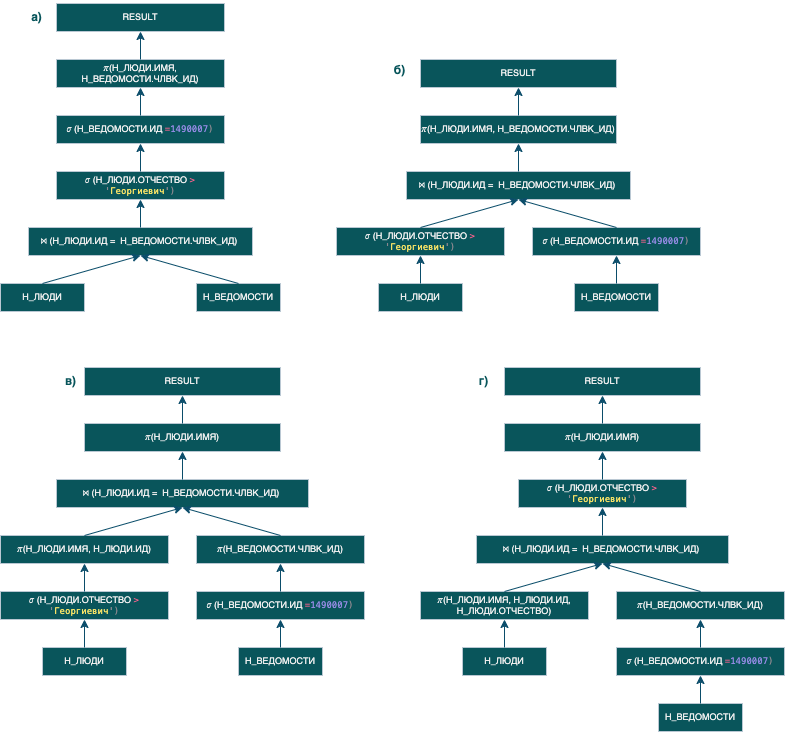
\includegraphics[width=\textwidth]{./image/plan-1.png}
Я считаю, что в общем случае оптимальным вариантом является план в) так, как объединяются только нужные строки и колонки (после выборки и проекции). 
Тем самым мы уменьшаем размер промежуточных данных => уменьшаем число операций чтения записи во внешнюю память.
\begin{lstlisting}
  QUERY PLAN
  -------------------------------------------
   Nested Loop  (cost=0.70..16.75 rows=1 width=17) (actual time=0.041..0.042 rows=0 loops=1)
     ->  Index Scan using "ВЕД_PK" on "Н_ВЕДОМОСТИ"  (cost=0.42..8.44 rows=1 width=4) (actual time=0.026..0.026 rows=1 loops=1)
           Index Cond: ("ИД" = 1490007)
     ->  Index Scan using "ЧЛВК_PK" on "Н_ЛЮДИ"  (cost=0.28..8.30 rows=1 width=17) (actual time=0.009..0.009 rows=0 loops=1)
           Index Cond: ("ИД" = "Н_ВЕДОМОСТИ"."ЧЛВК_ИД")
           Filter: (("ОТЧЕСТВО")::text > 'Георгиевич'::text)
           Rows Removed by Filter: 1
   Planning Time: 1.634 ms
   Execution Time: 0.115 ms
  (9 строк)
\end{lstlisting}
Мы видим, что Postgresql выбрал вариант г), так как в данном случае после выборки \\
Н\_ВЕДОМОСТИ.ИД осталась всего
одна строка. В таком случае меньше операций будет, если мы сначала соединим эту одну строку со строками Н\_ЛЮДИ (так как мы делаем RIGHT JOIN) и только потом отфильтруем Н\_ЛЮДИ.\\
В данном случае план не измениться после добавления индекса, но скорость выполнения увеличится.
\section{Запрос 2}
\subsection{Реализация запроса на SQL.}
\lstinputlisting[style=sql]{../src/query2.sql}
\begin{lstlisting}
  -- a) Индекс позволяет эффективно выбирать строки, основываясь на значении хеша столбца.
  CREATE INDEX Н_ЛЮДИ_ФАМИЛИЯ ON Н_ЛЮДИ USING HASH(ФАМИЛИЯ)
  -- б) Индекс позволяет эффективно выбирать строки, основываясь на их положении в дереве, а также так как выражения в WHERE отбираются с использованием знака >.
  CREATE INDEX Н_ВЕДОМОСТИ_ДАТА ON Н_ВЕДОМОСТИ USING BTREE(ДАТА)
  -- в) Индекс позволяет эффективно выбирать строки, основываясь на их положении в дереве, а также так как выражения в WHERE отбираются с использованием знака >.
  CREATE INDEX Н_СЕССИЯ_УЧГОД ON Н_СЕССИЯ USING BTREE(УЧГОД)
\end{lstlisting}
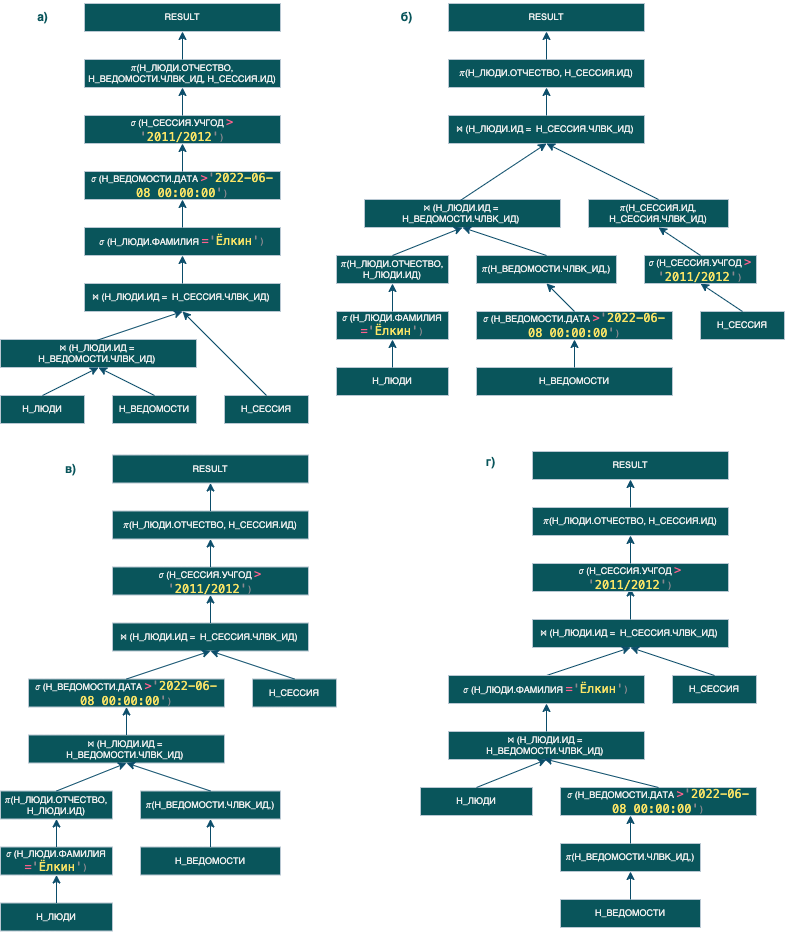
\includegraphics[width=\textwidth]{./image/plan-2.png}
В общем случае самым оптимальным был бы план б), но в данном случае если использовать план г) то после фильтрации ведомостей мы получим ноль строк и закончим выполнение раньше.\\
При добавлении предложенных индексов скорость выполнения увеличится и план г) все равно остается самым быстрым.
\begin{lstlisting}
  QUERY PLAN
  ---------------------------------------------
   Nested Loop  (cost=4.99..61.42 rows=1 width=28) (actual time=0.047..0.048 rows=0 loops=1)
     ->  Nested Loop  (cost=0.58..15.51 rows=1 width=28) (actual time=0.046..0.047 rows=0 loops=1)
           Join Filter: ("Н_ЛЮДИ"."ИД" = "Н_ВЕДОМОСТИ"."ЧЛВК_ИД")
           ->  Index Scan using "ФАМ_ЛЮД" on "Н_ЛЮДИ"  (cost=0.28..8.30 rows=1 width=24) (actual time=0.033..0.033 rows=1 loops=1)
                 Index Cond: (("ФАМИЛИЯ")::text = 'Ёлкин'::text)
           ->  Index Scan using "ВЕД_ДАТА_I" on "Н_ВЕДОМОСТИ"  (cost=0.29..7.20 rows=1 width=4) (actual time=0.009..0.010 rows=0 loops=1)
                 Index Cond: ("ДАТА" > '2022-06-08 00:00:00'::timestamp without time zone)
     ->  Bitmap Heap Scan on "Н_СЕССИЯ"  (cost=4.42..45.90 rows=1 width=8) (never executed)
           Recheck Cond: ("ЧЛВК_ИД" = "Н_ЛЮДИ"."ИД")
           Filter: (("УЧГОД")::text > '2011/2012'::text)
           ->  Bitmap Index Scan on "SYS_C003500_IFK"  (cost=0.00..4.42 rows=18 width=0) (never executed)
                 Index Cond: ("ЧЛВК_ИД" = "Н_ЛЮДИ"."ИД")
   Planning Time: 1.960 ms
   Execution Time: 0.142 ms
  (14 строк)
\end{lstlisting}
\section{Выводы по работе.}
В результате выполнения лабораторной работы были разработаны и проанализированы
два SQL запроса и планы их выполнения. В ходе выполнения были изучены особенности
составления и обработки планов СУБД PostgreSQL при использовании и без
использования индексов. Были изучены основные виды индексов и стратегии соединения
таблиц, применяемых в СУБД.
\end{document}
